%==============================================================================
% sections/04_dependent_cdmcs.tex
%==============================================================================
\section{Dependent Conditional Monte Carlo and Shock-Basis Extensions}
\label{sec:dependent-cdmcs}

\subsection{Exact CdMC identity under arbitrary dependence}

The first dependent extension is an identity. It does not require regular
variation, independence, or any factor structure; it only requires a regular
conditional distribution.

\begin{theorem}[Arbitrary-dependence selected-maximum CdMC identity]
\label{thm:dep-cdmc-unbiased}
Let \(X\in\RR^N\) have any joint distribution admitting regular conditional
laws. Fix a deterministic selected-maximum tie-breaking rule (\cref{ass:tie})
and define \(T_i(x)=(x-S_{-i})\vee M_{-i}\), with tie-rule endpoint
adjustments on null or discrete boundaries. Then
\[
  \Pb(S_N>x)
  =\sum_{i=1}^N
    \E\left[p_i(T_i(x);X_{-i})\right],
  \qquad
  p_i(t;X_{-i})=\Pb(X_i>t\mid X_{-i}).
\]
Consequently
\[
  Z^{\mathrm{dep}}(x)=\sum_{i=1}^N p_i(T_i(x);X_{-i})
\]
is an unbiased estimator of \(\mu(x)\) whenever the conditional kernels are
evaluated exactly.
\end{theorem}

\begin{proof}[Proof sketch]
Partition $\{S_N>x\}$ by the selected-maximum rule of \cref{ass:tie} into
disjoint events $E_i=\{S_N>x,R_i(X)=1\}$, each of which equals
$\{X_i>T_i(x)\}$ conditional on $X_{-i}$. Take expectations and sum. The full
argument and the population-identity / estimator distinction are in
\cref{appx:dependent-proofs}.
\end{proof}

\begin{remark}[What independence bought]
The independent estimator is the special case
\(p_i(t;X_{-i})=\Fb_i(t)\). Therefore independence is not the source of
unbiasedness. It is the source of a low-dimensional closed-form kernel and of
the deterministic envelope \(\sum_i\Fb_i(x/N)\). Under strong tail dependence,
the conditional kernel may become large on high-risk configurations and the
independent variance proof no longer applies.
\end{remark}

\subsection{A sufficient conditional-tail envelope for BRE}

A general arbitrary-dependence BRE theorem needs assumptions on conditional
survivals. The following condition is intentionally primitive; specialized
models below replace it by checkable shock-basis or radial assumptions.

\begin{assumption}[Conditional-tail envelope]
\label{ass:conditional-envelope}
There are nonnegative random variables \(K_{i,x}=K_{i,x}(X_{-i})\) and
deterministic functions \(b_i(x)\) such that, for all \(t\ge x/N\),
\[
  p_i(t;X_{-i})\le K_{i,x}b_i(t),
\]
where \(\sum_i b_i(x/N)=O(\mu(x))\) and
\[
  \E\left[\left\{\sum_{i=1}^N K_{i,x}b_i(x/N)\right\}^2\right]
  =O(\mu(x)^2).
\]
\end{assumption}

\begin{proposition}[BRE from a conditional-tail envelope]
\label{prop:dep-envelope-bre}
Under \cref{ass:conditional-envelope},
\[
  \sup_{x\ge x_0}
  \frac{\Var(Z^{\mathrm{dep}}(x))}{\mu(x)^2}<\infty
\]
for all sufficiently large \(x_0\).
\end{proposition}

\begin{proof}[Proof sketch]
$T_i(x)\ge x/N$ gives $Z^{\mathrm{dep}}(x)\le\sum_i K_{i,x}b_i(x/N)$, and the
second-moment envelope of \cref{ass:conditional-envelope} controls the
variance. The full argument is in \cref{appx:dependent-proofs}.
\end{proof}

\begin{remark}[Identifiability of conditional kernels]
\label{rem:kernel-identifiability}
The dependent CdMC identity invokes the conditional kernels
$p_i(t;X_{-i})$, which depend on the joint law of $X$. In practice these
kernels must either be derived in closed form from a parametric model (e.g.\ a
copula or latent-shock model) or estimated from data. Identifiability of the
kernel from observed data is not automatic: under strong tail dependence the
support of $X_{-i}$ relevant for the tail integral may be sparsely populated
in finite samples. The latent-shock, block, copula, MRV, and HRV
specializations developed below exist precisely to choose a more identifiable
conditioning object than the raw coordinatewise kernel.
\end{remark}

This proposition is useful as a diagnostic but not as a final model. It shows
why coordinatewise dependent CdMC can work under weak extremal dependence and
why it can fail under common shocks. If \(X_j\) is already extreme, the
conditional probability that \(X_i\) is also extreme may be much larger than
\(\Fb_i(t)\). In that regime the estimator should condition on the common shock,
block, or radial component instead.

\subsection{Copula and vine implementation of the exact kernel}

If \(U_i=F_i(X_i)\) and \(U\) has copula \(C\), then the exact kernel is
\[
  p_i(t;X_{-i})
  =1-C_{i\mid -i}\{F_i(t)\mid U_{-i}\}.
\]
For elliptical, Archimedean, and vine copulas this conditional distribution can
be computed by standard conditional copula formulas or by vine h-functions.
The planned copula estimator is therefore
\[
  Z^{\mathrm{cop}}(x)=\sum_{i=1}^N
  \left[1-C_{i\mid -i}\{F_i(T_i(x))\mid U_{-i}\}\right].
\]
The simulation section tests this estimator in Gaussian, \(t\), Clayton,
Gumbel, and vine designs. The real-data section uses it only after reporting
marginal tail and copula-tail diagnostics, because misspecified copulas can be
precisely wrong in the region that matters.

\subsection{Latent independent shocks}

Suppose observed factors are dependent because they are linear combinations of
independent shocks:
\[
  F=BZ, \qquad Z_1,\ldots,Z_K\ \text{independent}.
\]
For portfolio exposure \(a\), define \(q=B^\top a\), so \(L=a^\top F=q^\top Z\).
Let \(Z_k\) have right and left tail constants \(p_k^+,p_k^-\) relative to
\(\Gb\). The active shock constant is
\[
  c_k(q_k)=|q_k|^\alpha\{p_k^+\1(q_k>0)+p_k^-\1(q_k<0)\}.
\]

\begin{theorem}[Latent-shock tail constant]
\label{thm:latent-shock-tail}
Assume the shocks \(Z_1,\ldots,Z_K\) are independent and satisfy the
independent single-big-jump assumptions after signing by \(q_k\). Then
\[
  \Pb(q^\top Z>x)
  \sim \Gb(x)\sum_{k=1}^K c_k(q_k).
\]
Moreover the independent CdMC estimator applied to the shock contributions
\(q_kZ_k\) is unbiased and has the independent BRE bound with \(K\) in place of
\(N\), or with the number of active shocks after active-only stratification.
\end{theorem}

\begin{proof}[Proof sketch]
Apply \cref{thm:sum-equivalence} to the independent signed shock contributions
$Y_k=q_kZ_k$. The full argument is in \cref{appx:dependent-proofs}.
\end{proof}

The theorem is elementary but consequential: the unit of tail attribution is a
latent shock, not necessarily an observed factor.

\begin{example}[Common shock]
\label{ex:common-shock}
Let \(X_i=b_iZ_0+E_i\), where \(Z_0,E_1,\ldots,E_N\) are independent and
regularly varying with common index. Then
\[
  S_N=\left(\sum_{i=1}^N b_i\right)Z_0+
      \sum_{i=1}^N E_i.
\]
The common-shock contribution to the leading right tail is proportional to
\((\sum_i b_i)_+^\alpha\). Treating the observed \(X_i\)'s as independent would
instead create a term proportional to \(\sum_i (b_i)_+^\alpha\), which can be
severely wrong when the exposures have the same sign.
\end{example}

\begin{figure}[t]
\centering
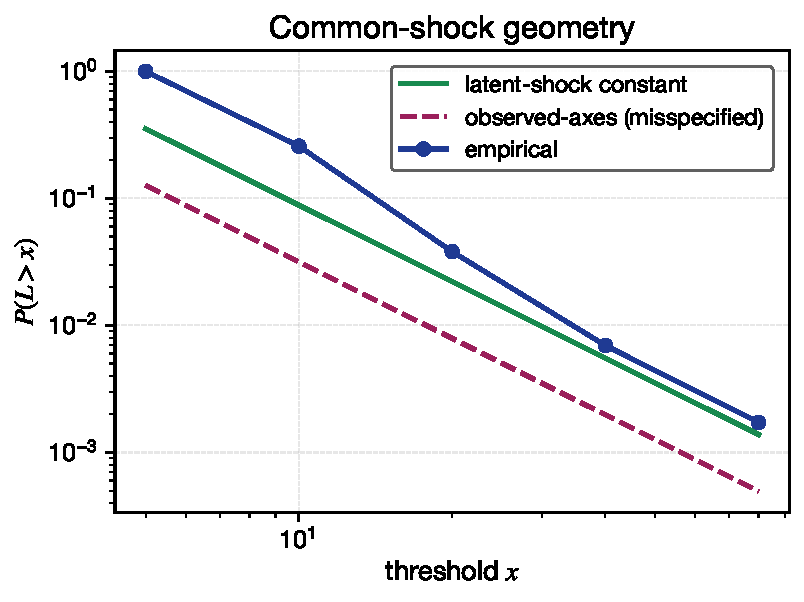
\includegraphics[width=0.85\linewidth]{figures/F11_common_shock_geometry.pdf}
\caption[Common-shock tail geometry]{Empirical sum-tail of $X = bZ_0 + E$ (blue) compared with the latent-shock constant (green) and the misspecified observed-axes constant (dashed purple). The empirical tail tracks the latent constant; the observed-axes constant under-states the tail by $\sim 2.8\times$.}
\label{fig:common-shock-geometry}
\end{figure}


\subsection{Block-dependent aggregation}

Let \(\{1,\ldots,N\}=B_1\cup\cdots\cup B_K\) be a partition. Define block sums
\(Y_k=\sum_{i\in B_k}X_i\). Assume the blocks are independent, while dependence
inside each block is arbitrary.

\begin{theorem}[Independent-block reduction]
\label{thm:block-reduction}
If \(Y_1,
\ldots,Y_K\) are independent and
\[\Pb(Y_k>x)\sim d_k\Gb(x),\]
and the block sums satisfy the finite single-big-jump conditions, then
\[
  \Pb(S_N>x)=\Pb\left(\sum_{k=1}^KY_k>x\right)
  \sim \sum_{k=1}^K\Pb(Y_k>x)
  \sim \left(\sum_{k=1}^K d_k\right)\Gb(x).
\]
\end{theorem}

\begin{proof}[Proof sketch]
Apply \cref{thm:sum-equivalence} to the independent block sums. The full
argument is in \cref{appx:dependent-proofs}.
\end{proof}

In financial applications, blocks may be sectors, regions, liquidity buckets,
volatility regimes, or factors grouped by empirical tail dependence. The block
constant \(d_k\) can be estimated by within-block MRV, a common-shock model, a
copula estimator, or high-precision simulation.

\begin{remark}[Numerical stability of conditional-kernel evaluation]
\label{rem:numerical-stability}
When the conditional kernel $p_i(t;X_{-i})$ is computed from a closed-form
survival expression that is under-flow prone at large $t$ (for example,
Gaussian or Student-$t$ conditional tails at the 99.9\% quantile), the kernel
should be evaluated on log-scale: compute $\log p_i$ via Mills'-ratio or
asymptotic series and exponentiate at the last step. Sum-of-kernel estimators
$Z^{\mathrm{dep}}(x)=\sum_i p_i(T_i;X_{-i})$ then aggregate the
exponentiated quantities; if any single kernel under-flows to zero, the
log-sum-exp identity may be used at the outer level to retain accuracy in the
overall estimator.
\end{remark}

\subsection{Estimator decision point}

The practical decision is not whether dependence exists; it does. The decision
is whether dependence changes the first-order constant materially at the
thresholds of interest. The paper therefore uses the workflow in
\cref{fig:estimator-decision-tree}: start with marginal tails, test tail
dependence and spectral concentration, choose independent/latent/block/copula
or MRV estimator, then backtest VaR and ES out of sample.

\begin{figure}[t]
\centering
\begin{tikzpicture}[
  node distance=0.65cm and 0.9cm,
  box/.style={rectangle, rounded corners, draw, align=center, minimum width=2.7cm, minimum height=0.8cm, font=\scriptsize},
  decision/.style={diamond, aspect=2.2, draw, align=center, font=\scriptsize, inner sep=1pt},
  arr/.style={->, >=Stealth}
]
\node[box, fill=blue!10] (data) {Signed loss\\contributions};
\node[decision, fill=yellow!15, right=of data] (marg) {Common heavy\\tail scale?};
\node[box, fill=red!8, above right=of marg] (fixmarg) {Use heterogeneous\\tail model};
\node[decision, fill=yellow!15, below right=of marg] (taildep) {Extremal\\dependence?};
\node[box, fill=green!12, below left=of taildep] (ind) {Independent\\CdMC};
\node[decision, fill=yellow!15, right=of taildep] (geom) {Geometry stable?};
\node[box, fill=green!12, above right=of geom] (latent) {Latent/block\\CdMC};
\node[box, fill=green!12, right=of geom] (spec) {Spectral\\CdMC};
\node[box, fill=green!12, below right=of geom] (hidden) {Hidden-cone\\mixture};
\draw[arr] (data) -- (marg);
\draw[arr] (marg) -- node[above, font=\scriptsize] {no} (fixmarg);
\draw[arr] (marg) -- node[left, font=\scriptsize] {yes} (taildep);
\draw[arr] (taildep) -- node[left, font=\scriptsize] {weak} (ind);
\draw[arr] (taildep) -- node[above, font=\scriptsize] {yes} (geom);
\draw[arr] (geom) -- node[left, font=\scriptsize] {rays/blocks} (latent);
\draw[arr] (geom) -- node[above, font=\scriptsize] {full MRV} (spec);
\draw[arr] (geom) -- node[right, font=\scriptsize] {axis first order} (hidden);
\end{tikzpicture}

\caption[Estimator decision tree]{Estimator decision tree for dependent factor
risk. The tree is used both in simulation and in the real-data analysis. It is a
model-selection protocol, not a claim that one estimator dominates universally.}
\label{fig:estimator-decision-tree}
\end{figure}
